\documentclass[a4paper, 10pt]{article}
\usepackage{graphics, a4wide, graphicx,enumerate}
\usepackage{nopageno}
\usepackage{txfonts}
\usepackage[usenames]{color}

\title{Second Order Navier Stokes Solvers for Vortex Solutions in Lid-Driven Cavities}
\author{Girish Nivarti}
\date{\today}

\begin{document}
\maketitle
\begin{enumerate}[I]

\item The $L_2$ norms of error in flux integrals have been tabulated for various meshes in Table \ref{norm}. The errors in approximation to equation 1 (in Problem Sheet) have been tabulated for a 10x10 mesh in Table \ref{jacobian}. Spurious errors due to round-off were observed in even exact solution values. This, however, did not effect the significant digits in the error (where such spurious errors were seen at less significant digits).
\begin{table}
\begin{center}
\begin{tabular}{|l | r | r | r |}
\hline
Mesh Size & Error ($U_1$) & Error ($U_2$) & Error ($U_3$) \\
\hline
10 $\times$ 10 & 0.0479469 & 0.195058 & 0.195058 \\
20 $\times$ 20 & 0.0119834 & 0.0500259 & 0.0500259 \\
40 $\times$ 40 & 0.0029957 & 0.0125859 & 0.0125859 \\
80 $\times$ 80 & 0.000748916 & 0.00315144 & 0.00315144 \\
\hline
\end{tabular}
\caption{$L_2$ Norms of error in flux integral for solution with $P_0$, $u_0$, $v_0$, and $\beta$ set to 1.0, and $Re = 10$.}
\label{norm}
\end{center}
\end{table}

\begin{table}
\begin{center}
\begin{tabular}{|l | r | r | r |}
\hline
Cell Location & Error ($U_1$) & Error ($U_2$) & Error ($U_3$) \\
\hline
10, 09 & 1.00018e-17 & 4.99997e-12 & 4.99994e-12 \\
09, 10 & 1.00018e-17 & 4.99994e-12 & 5.00008e-12 \\
10, 10 & 0 & 1.00668e-16 & 1.00668e-16 \\
11, 10 & -1.00018e-17 & -4.99998e-12 & -4.99987e-12 \\
10, 11 & -1.00018e-17 & -4.99987e-12 & -4.99998e-12 \\
\hline
\end{tabular}
\caption{Approximation error in change in flux integral with time step.}
\label{jacobian}
\end{center}
\end{table}
\begin{table}
\begin{center}
\begin{tabular}{|l | r | r | r |}
\hline
Cell Location & Error ($U_1$) & Error ($U_2$) & Error ($U_3$) \\
\hline
\[9\]\[9\] & 0 & 0 & 0 \\
\[10\]\[9\] & 2.54801e-16 & 2.5e-12 & 2.49998e-12 \\
\[9\]\[10\] & -1.89288e-16 & 2.49998e-12 & 2.50006e-12 \\
\[10\]\[10\] & 0 & -1.25988e-17 & -1.25988e-17 \\

\item Following are observations and relevant illustrations from the experiments on optimizing the code. The following results were achieved with $Re = 100$, ona  20x20 mesh.
  \begin{enumerate} [a]
  \item No pressure drift was observed in the solution. The pressure solution converged for a variety of parameters and Reynolds numbers, and hence no fixed boundary condition was applied for pressure at a single ghost cell. 
    \item To reduce pressure oscillations due to coupling of pressure in alternate lines of the mesh, a laplacian term ($A\Delta x \Delta y \nabla P$)of pressure was introduced in the continuity (pressure) equation.  The value of A was varied to observe different results of smoothening as shown in Fig. \ref{smooth}, and Fig. \ref{smooth2} where slices of mesh with most oscillations ($i = 11$, and $j = 11$) have been plotted. 
    \item The weight ($\beta$) given to transient pressure term in the continuity equation was varied to observe effects on convergence rate. Similarly successive over-relaxation coefficient ($\omega$), and time steps were tuned to give optimum convergence. The individual effects of each of these independent of other parameters have been tabulated in Table \ref{tune}.

\begin{figure}
  \centering
  \includegraphics[width=0.6\textwidth, angle = -90]{../plot/oscillation/osc.eps}
  \caption{Pressure oscillations are damped along the x direction by adding a diffusion term. A = 0.1 gives best results.}
  \label{smooth}
\end{figure}

\begin{figure}
  \centering
  \includegraphics[width=0.6\textwidth, angle = -90]{../plot/oscillation/osci.eps}
  \caption{Pressure oscillations are damped along the y direction by adding a diffusion term. A = 0.1 gives best results.}
  \label{smooth2}
\end{figure}

\begin{table}
\begin{center}
\begin{tabular}{| l | r || r | r || r | r |}
\hline
$\beta$ & Iterations & $\omega$ & Iterations & $\Delta t$ & Iterations\\
\hline

0.5 & 232 & 1.0 & 256 & 0.05 & 256\\
0.6 & 228 & 1.1 & 246 & 0.10 & 151\\ \cline{1-2}
0.7 & 224 & 1.2 & 238 & 0.15 & 123\\ \cline{1-2}
0.8 & 236 & 1.3 & 231 & 0.20 & 110\\ \cline{5-6}
0.9 & 249 & 1.4 & 226 & 0.25 & 103\\ \cline{3-4} \cline{5-6}
1.0 & 256 & 1.5 & 224 & 0.30 & 99\\ \cline{3-4}
1.2 & 281 & 1.6 & 225 & 0.35 & 98\\
1.3 & n/a & 1.7 & 224 & 0.40 & 98\\
1.4 & n/a & 1.8 & 228 & 0.45 & 100\\

\hline
\end{tabular}
\caption{Convergence behaviour of solution observed on independently varying $\beta$, successive-over-relaxation parameter $\omega$, and time step $\Delta t$, with a fixed $Re = 100$ for a mesh size of 20 $\times$ 20. The optimal parameters chosen for later excercises have been highlighted.}
\label{tune}
\end{center}
\end{table}
%% Solution with beta: 1.2 converged to 9.11969533183182e-07  4.27979481936932e-07  7.2030130338805e-07 in 281 steps
%% Solution with beta: 1 converged to 9.44301326316753e-07  3.29472861330548e-07  8.78914671830617e-07 in 256 steps
%% Solution with beta: 0.9 converged to 3.67014055208618e-07  2.17094389384209e-07  9.22635635110267e-07 in 249 steps
%% Solution with beta: 0.8 converged to 5.32603833158466e-07  3.79660412609399e-07  9.59216144769778e-07 in 236 steps
%% Solution with beta: 0.7 converged to 5.7496360264576e-07  9.63583958358859e-07  9.38262426101032e-07 in 224 steps
%% Solution with beta: 0.6 converged to 8.37903257343103e-08  8.92256293049541e-07  9.89176926409004e-07 in 228 steps
%% Solution with beta: 0.5 converged to 2.74084747758119e-08  9.69284617250733e-07  9.75559531615711e-07 in 232 steps

 %% Solution with SOR: 2.2 converged to 9.37015914510813e-07  6.99745225715309e-07  5.38951653500861e-07 in 366 steps
 %% Solution with SOR: 2.1 converged to 8.06081010694755e-07  9.06657874342554e-07  7.08664976911585e-07 in 266 steps
 %% Solution with SOR: 2 converged to 3.52965190658196e-07  9.77040931079523e-07  9.95741947933958e-07 in 242 steps
 %% Solution with SOR: 1.9 converged to 8.41119887293313e-07  9.06189431314842e-07  8.94752323482843e-07 in 232 steps
 %% Solution with SOR: 1.8 converged to 6.62078737273958e-07  8.85821127353255e-07  8.83502748906094e-07 in 228 steps
 %% Solution with SOR: 1.7 converged to 7.63752004364419e-07  8.56181711890409e-07  8.81869584441157e-07 in 224 steps
 %% Solution with SOR: 1.6 converged to 8.6726066816062e-07  7.68110149095951e-07  6.78370720654392e-07 in 225 steps
 %% Solution with SOR: 1.5 converged to 6.28665567737143e-07  8.88136285772826e-07  7.33122430161234e-07 in 224 steps
 %% Solution with SOR: 1.4 converged to 6.86199414470014e-07  7.45339346361567e-07  9.27149817416412e-07 in 226 steps
 %% Solution with SOR: 1.3 converged to 9.18378100467231e-07  7.74520331296658e-07  4.92195173193926e-07 in 231 steps
 %% Solution with SOR: 1.2 converged to 8.67562966360854e-07  4.16687947760643e-07  7.54767341423407e-07 in 238 steps
 %% Solution with SOR: 1.1 converged to 9.17431140778705e-07  7.85877821735947e-07  3.3126458863817e-07 in 246 steps
 %% Solution with SOR: 1 converged to 9.44301326316753e-07  3.29472861330548e-07  8.78914671830617e-07 in 256 steps

 %% Solution with dt: 0.05 converged to 9.44301326316753e-07  3.29472861330548e-07  8.78914671830617e-07 in 256 steps
 %% Solution with dt: 0.1 converged to 2.47494716683907e-08  9.85919833493916e-07  9.85086072684939e-07 in 151 steps
 %% Solution with dt: 0.15 converged to 2.50100012627708e-08  9.81679910491457e-07  9.80037618474944e-07 in 123 steps
 %% Solution with dt: 0.2 converged to 2.98101853069845e-08  9.29042848628983e-07  9.26202521823676e-07 in 110 steps
 %% Solution with dt: 0.25 converged to 4.01950649933332e-08  9.26968145563461e-07  9.22515279165748e-07 in 103 steps
 %% Solution with dt: 0.3 converged to 5.58472798473289e-08  9.72979538606726e-07  9.66272070560794e-07 in 99 steps
 %% Solution with dt: 0.35 converged to 7.11019303920279e-08  9.51116611327209e-07  9.41999138501301e-07 in 98 steps
 %% Solution with dt: 0.4 converged to 9.72488484658789e-08  9.96865386563812e-07  9.83193882833143e-07 in 98 steps
 %% Solution with dt: 0.45 converged to 1.24455702558706e-07  9.98367287571365e-07  9.79084118223986e-07 in 100 steps


  \end{enumerate}

\item The validation case of a square domain with moving top is explored here. The following results have been achieved without using the tuned parameters arrived at in the previous section. This was due to the fact that most of the parameters were mentioned explicitly in the question. Hence, $Re = 100$, $\beta = 1$, $A = 0$ have been used on a 20x20 mesh. Over-relaxation $\omega = 0$, and times step $\Delta t = 0.05$ were, however, varied as asked and have been reported accordingly. Convergence criterion used is for the $L_2$ norm of change in solution to be less than $10^{-6}$.
  \begin{enumerate} [a]
  \item Convergence history of solution with zero lide velocity has been plotted in Fig. \ref{ch1}. Alongside, steady state contour plots of pressure, and velocities have been plotted (Figures \ref{sol1p}, \ref{sol1u}, \ref{sol1v})to verify that the solution indeed reaches the stable values expected. There were minor oscillations in steady state pressure due to the lack of tuning parameter A. The average (over entire domain) values of respective fields were calculated as 1.9519992854088 $\times 10^{-15}$, -1.34855056741173 $\times 10^{-17}$, -2.90050021523882 $\times 10^{-17}$. An over-relaxation coefficient ($\omega = 1.5$) was used to attain convergence in 224 steps.
  \item On a 20x20 mesh, results of using a driven lid ($U_{top} = 1$) have been shown here. The convergence history has been plotted until convergence was attained (Fig. \ref{ch2}, \ref{ch3}, \ref{ch4}). Velocity in x-direction has been plotted for both cases ($U_{top} = 1$ and $U_{top} = -1$), as comparison, along the vertical line of symmetry in Fig. \ref{uvel}. A surface plot of pressure has been provided (Fig. \ref{splotP}) alongside.
  \item In order to guarantee symmetry in solutions of forward, and backward driven lids, a surface plot of $u_{U_{top} = 1}(x,y) + u_{U_{top} = -1}(1-x,y)$ has been constructed (Fig. \ref{splotU}).
  \item Grid convergence has been established by successively refining the mesh, and plotting velocity (Fig. \ref{Ugci}) along the symmetry line for each case. For a quantitative reasoning, norms of change in solution across two successive meshes at 10 different points (those from the smallest mesh) were calculated, and plotted (Fig. \ref{dUgci}). An 160x160 mesh is sufficient for grid convergence.
  \end{enumerate}
  
  
\item
  
  \begin{figure}
    \centering
    \includegraphics[width=0.6\textwidth, angle = -90]{../plot/stability/convergence/conv.eps}
    \caption{Change in solution (in pressure, and velocities) plotted over iterations up to 200 iterations.}
    \label{ch1}
    \end{figure}
  
  \begin{figure}
      \centering
      \includegraphics[width=0.6\textwidth, angle = -90]{../plot/stability/solution/P.eps}
      \caption{Steady state pressure contour plot for a 20x20 mesh with no lid velocity.}
      \label{sol1p}
    \end{figure}
    \begin{figure}
      \centering
      \includegraphics[width=0.6\textwidth, angle = -90]{../plot/stability/solution/u.eps}
      \caption{Steady state x velocity (u) contour plot for a 20x20 mesh with no lid velocity.}
      \label{sol1u}
    \end{figure}
    \begin{figure}
      \centering
      \includegraphics[width=0.6\textwidth, angle = -90]{../plot/stability/solution/v.eps}
      \caption{Steady state y velocity (v) contour plot for a 20x20 mesh with no lid velocity.}
      \label{sol1v}
    \end{figure}

    
    \begin{figure}
      \centering
      \includegraphics[width=0.6\textwidth, angle = -90]{../plot/basic/convergence/convP.eps}
      \caption{Convergence history of pressure for a forward driven lid case in a square mesh for different combinations of $\Delta t$, and $\omega$.}
      \label{ch2}
    \end{figure}
    \begin{figure}
      \centering
      \includegraphics[width=0.6\textwidth, angle = -90]{../plot/basic/convergence/convU.eps}
      \caption{Convergence history of x velocity for a forward driven lid case in a square mesh for different combinations of $\Delta t$, and $\omega$.}
      \label{ch3}
    \end{figure}

    \begin{figure}
      \centering
      \includegraphics[width=0.6\textwidth, angle = -90]{../plot/basic/convergence/convV.eps}
      \caption{Convergence history of y velocity for a forward driven lid case in a square mesh for different combinations of $\Delta t$, and $\omega$.}
      \label{ch4}
    \end{figure}
    
    \begin{figure}
      \centering
      \includegraphics[width=0.6\textwidth, angle = -90]{../plot/basic/symmetry/uvel.eps}
      \caption{Plot of u along the vertical line of symmetry for both froward, and backward driven cases.}
      \label{uvel}
    \end{figure}
    
    \begin{figure}
      \centering
      \includegraphics[width=0.6\textwidth, angle = -90]{../plot/basic/pressure/P.eps}
      \caption{Surface plot of pressure for the forward driven case.}
      \label{splotP}
    \end{figure}
    
    \begin{figure}
      \centering
      \includegraphics[width=0.6\textwidth, angle = -90]{../plot/basic/velocity/UU.eps}
      \caption{Surface plot of pressure for the forward driven case. Values do not attain exact zeros due to lack of complete iterative convergence.}
      \label{splotU}
    \end{figure}

    \begin{figure}
      \centering
      \includegraphics[width=0.6\textwidth, angle = -90]{../plot/basic/gci/gci.eps}
      \caption{Plot of velocity along vertical line of symmetry for different meshes.}
      \label{Ugci}
    \end{figure}

    \begin{figure}
      \centering
      \includegraphics[width=0.6\textwidth, angle = -90]{../plot/basic/gci/gci2.eps}
      \caption{Plot of change in velocity estimate along vertical line of symmetry between different meshes. The $L_2$ norms of these changes were calculated as 0.0210647, 0.00686623, 0.00188125, and 0.000458044. The changes are diminishingly small, and smaller by a factor of four for the 160x160 mesh.}
      \label{dUgci}
    \end{figure}

\end{enumerate}
%\input{../plot/stability/conv}

%% %Sec 3.1


%% %sec 3.2.1, 3.2.2
%% dt = 0.05
%% U = 1.0:  Solution with SOR: 1 converged to 9.6660720727693e-07  9.96190587746852e-07  4.65312262596864e-07 in 413 steps Code run time = 10000 ms
%% U = -1: Solution with SOR: 1 converged to 9.5485765470563e-07  9.47307751656132e-07  1.47032202389875e-07 in 399 steps Code run time = 10000 ms

%% dt = 0.05
%%  Solution with SOR: 1.5 converged to 9.33931991223728e-07  9.58859204246978e-07  5.84482577033519e-07 in 392 steps Code run time = 9000 ms

%% dt = 0.25
%%  Solution with SOR: 1 converged to 2.76747563529065e-07  9.70727396324067e-07  9.0256255090202e-07 in 88 steps Code run time = 2000 ms

%% dt = 0.25
%%  Solution with SOR: 1.5 converged to 2.59031812762338e-07  8.93762114854779e-07  8.26267053540912e-07 in 63 steps Code run time = 1000 ms
%%  Solution with SOR: 1.5 converged to 2.62338962584223e-07  9.08122099312736e-07  8.36681047064573e-07 in 76 steps Code run time = 1000 ms

%% %3.2.3


%% %4.1

\end{document}
